
\section{Architekturänderung}

Im Folgenden wird die Planung und Implementierung der Architekturänderung zwecks Entkopplung der Z3-Komponente aus ProB beschrieben.

\subsection{Planung}

Um eine korrekte Systemrefaktorisierung durchzuführen, ist es notwendig, zuvor grundlegende Kernaspekte
des neuen Systems vollständig zu planen. Dies beinhaltet insbesondere die Struktur des neuen Server-Prozesses
und den Aufbau der Nachrichten, die zwischen den Prozessen ausgetauscht werden.

\subsubsection{Prolog Datentypen}

Innerhalb des bestehenden Z3-Interfaces werden verschiedene Prolog-Datentypen verwendet.
Da durch die Entkopplung der Prozesse Prolog selbst und die Z3-Komponente nicht länger direkt miteinander kommunizieren können,
müssen die Prolog-Datentypen in eine Form umgewandelt werden, die über das Netzwerk übertragen werden kann und von Z3 verstanden wird.

Primär werden die folgenden Prolog-Datentypen verwendet: \texttt{SP\_atom}, \texttt{SP\_integer} und \texttt{SP\_term\_ref}.
Mithilfe des Foreign Function Interface (FFI) von SICStus Prolog \cite{carlsson1988sicstus}, das durch die Header-Datei \texttt{sicstus/sicstus.h} bereitgestellt wird, können diese Datentypen konvertiert werden.
So stehen bei der Umwandlung von \texttt{SP\_atom} in einen C\texttt{++} String die Funktionen \texttt{SP\_string\_to\_atom} und \texttt{SP\_atom\_to\_string} zur Verfügung.
Die Dokumentation von SICStus Prolog schlägt unter dem Kapitel \enquote{Conversions between Prolog Arguments and C Types} zudem zur Umwandlung von \texttt{SP\_integer} den Datentyp C long vor.
Der Typ \texttt{SP\_term\_ref} wird in der Dokumentation wie folgt beschrieben: \enquote{The argument could be any term.}.
Insbesondere ist zu beachten, dass dies auch iterierbare Datentypen wie Listen oder Sets umfasst, welche dekonstruiert werden müssen, um an die enthaltenen Elemente zu gelangen.
\texttt{SP\_term\_ref} lässt sich also nur schwer gezielt in einen C\texttt{++} Datentyp umwandeln und muss daher mit besonderer Vorsicht behandelt werden.
Dies geschieht durch die Verwendung von speziellen (Hilfs-)Funktionen, welche die Prolog-Terme explizit kategorisieren und gegebenfalls in ihre Bestandteile zerlegen.

Zusätzlich existiert keine klare Struktur zur Behandlung dieser Prolog-Datentypen im Code,
da die Funktionen zur Datenextraktion verstreut vorliegen und nicht zentralisiert sind.
Es wird also global davon ausgegangen, dass der SICStus-Kontext verfügbar ist, was zu einer impliziten Kopplung führt, da keine Isolation der Prolog-Logik stattfindet.

\subsubsection{Struktur der Nachrichten}
\todo{Einbinden der grapfik, formale definitionen, besserer text}
Innerhalb von ZeroMQ lassen sich verschiedene Datenwerte gemeinsam in einen Nachrichtenblock packen.
Ein solcher Nachrichtenblock wird über das abstrakte \texttt{zmsg\_t} Objekt repräsentiert, welches es ermöglicht,
komplexere Daten zusammen in sogenannten Frames zu übermitteln.
Da sich der konkrete Inhalt der Nachrichten je nach Interfacefunktion unterscheidet,
bietet es sich an, dieses Konzept zu nutzen und den Inhalt spezifisch für jede Funktion zu definieren und zu interpretieren.

Zusätzlich zu den eigentlichen Daten, die übermittelt werden, ist es jedoch notwendig, Metadaten zu übermitteln,
die die korrekte Interpretation der Nachrichten auf der Empfängerseite ermöglichen.
Wenn eine Anfragenachricht von ProB an den Z3-Server gesendet wird, muss der Server wissen, welche Funktion aufgerufen werden soll.
Dafür wird ein Funktionsidentifikator benötigt, der die Funktion eindeutig identifiziert.
Diese Identifikatoren werden als ein Enum-Typ definiert, der die verschiedenen Funktionen als Konstanten repräsentiert und in sowohl
der ProB- als auch der Z3-Komponente eingebunden wird.
Ein Ausschnitt des Enum-Typs ist in \cref{lst:func-identifiers} gezeigt.

\begin{lstlisting}[
    float, caption={Ein Ausschnitt des Funktionsidentifikations-Enums.}, label={lst:func-identifiers}, language=C++
  ]
  enum SP_Function {
    INIT = 0,
    PRETTY_PRINT_SMT = 1,
    PRETTY_PRINT_SMT_FOR_ID = 2,
    MK_VAR = 3,
    // ...
  }
\end{lstlisting}

Wenn eine Antwortnachricht vom Z3-Server an ProB gesendet wird, muss die Nachricht ebenfalls Metadaten enthalten,
die die korrekte Interpretation der Nachricht auf der ProB-Seite ermöglicht.
Dafür wird ein Statusidentifikator benötigt, der den Status der Anfrage repräsentiert.
Der hierfür verwendete Enum-Typ ist in \cref{lst:status-identifiers} gezeigt.

\begin{lstlisting}[
    float, caption={Das Statusidentifikations-Enum.}, label={lst:status-identifiers}, language=C++
  ]
  enum Z3Status {
    NOK,
    OK,
    UNFINISHED
  }
\end{lstlisting}

\begin{figure}[!htp]
    \centering
    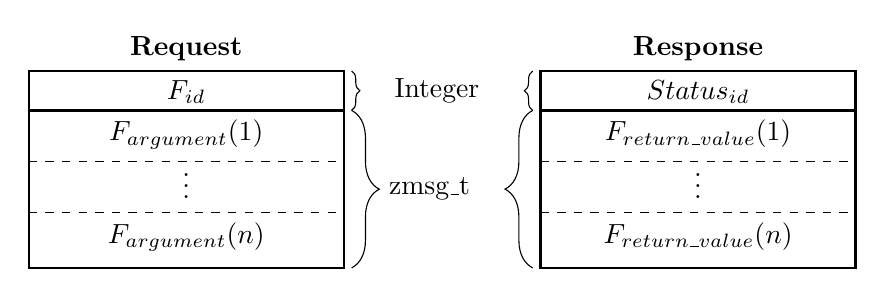
\begin{tikzpicture}[scale=1, every node/.style={scale=1}]
        % Request box
        \node[above] at (2, 2.5) {\textbf{Request}};
        \draw[thick] (0, 2.5) rectangle (4, 0);
        \node[below] at (2, 2.5) {$F_\text{id}$};
        \draw[thick] (0, 2) -- (4, 2);
        \node[below] at (2, 2) {$F_\text{argument}(1)$};
        \draw[dashed] (0, 1.35) -- (4, 1.35);
        \node[below] at (2, 1.53) {$\vdots$};
        \draw[dashed] (0, 0.7) -- (4, 0.7);
        \node[below] at (2, 0.7) {$F_\text{argument}(n)$};
        \draw[decorate, decoration={brace, amplitude=10pt}] (4.1, 2) -- (4.1, 0)
            node[midway, right=10pt] {\text{zmsg\_t}};
        \draw[decorate, decoration={brace, amplitude=3pt}] (4.1, 2.5) -- (4.1, 2)
            node[midway, right=12pt] {\text{Integer}};
        % Response box
        \node[above] at (8.5, 2.5) {\textbf{Response}};
        \draw[thick] (6.5, 2.5) rectangle (10.5, 0);
        \node[below] at (8.5, 2.5) {$Status_\text{id}$};
        \draw[thick] (6.5, 2) -- (10.5, 2);
        \node[below] at (8.5, 2) {$F_\text{return\_value}(1)$};
        \draw[dashed] (6.5, 1.35) -- (10.5, 1.35);
        \node[below] at (8.5, 1.53) {$\vdots$};
        \draw[dashed] (6.5, 0.7) -- (10.5, 0.7);
        \node[below] at (8.5, 0.7) {$F_\text{return\_value}(n)$};
        \draw[decorate, decoration={brace, amplitude=10pt}] (6.4, 0) -- (6.4, 2);
        \draw[decorate, decoration={brace, amplitude=3pt}] (6.4, 2) -- (6.4, 2.5);

    \end{tikzpicture}
    \caption{Das Kommunikationsprotokoll zwischen Client und Server.}
    \label{fig:protocol}
\end{figure}

Die Statuswerte \texttt{OK} und \texttt{NOK} repräsentieren den Erfolg oder Misserfolg einer Anfrage.
Diese Werte sind fundamental, da bei dem Aufkommen von potenziellen Fehlern oder Exceptions (siehe \cref{subsec:exceptions}) in Z3 der ProB Prozess über den Misserfolg informiert werden muss,
um eine entsprechende Fehlerbehandlung durchzuführen.
Der Statuswert \texttt{UNFINISHED} wird verwendet, wenn eine Anfrage noch nicht abgeschlossen ist und der Server auf weitere Informationen wartet (siehe \cref{subsec:helper-functions}).

Insgesamt besteht eine Nachricht also immer aus einem Identifikator (von Typ Integer), der entweder eine Funktion oder einen Status repräsentiert,
gefolgt von den eigentlichen Daten, die übermittelt werden sollen, in Form eines \texttt{zmsg\_t} Objektes.

\subsubsection{Server Struktur}

Da sich der Z3-Server aktuell mit nur einem einzigen Client beschäftigen muss,
bieten sich die ZeroMQ Kommunikationsmuster \enquote{Request-Reply} oder \enquote{Pair-Pair} an.
Da jedoch der Prozess des Lösens eines Prädikates abhängig von den vorherigen Arbeitsschritten ist,
bietet das synchrone Kommunikationsmuster \enquote{Request-Reply} die beste Lösung, ohne dem System unnötige Komplexität hinzuzufügen.
Bei dem gewählten Muster ist zu beachten, dass eine strikte Reihenfolge der Nachrichten eingehalten werden muss.
Angefangen bei der ersten Request Nachricht ausgehend von ProB müssen sich die Nachrichten abwechseln, um eine korrekte Kommunikation zu gewährleisten.
Dies ist im Kontrollfluss der Anwendungen zu berücksichtigen, um Deadlocks oder anderweitige Probleme zu vermeiden.

Innerhalb der Entwicklungsumgebung wird der entkoppelte Solver auf demselben Rechner ausgeführt,
weshalb IPC als Kommunikationsprotokoll verwendet wird, um eine effiziente und schnelle Kommunikation über das Dateisystem zu gewährleisten.
Das eigentliche Protokoll lässt sich jedoch innerhalb der ZeroMQ Bibliothek leicht konfigurieren, sodass zukünftig auch eine verteilte Systemarchitektur möglich ist.

Die Kernlogik des Servermodells ist simpel gehalten.
Nach dem Instanziieren des Sockets wird eine Endlosschleife gestartet, die auf eingehende Nachrichten wartet.
Sobald eine Nachricht empfangen wird, wird zunächst der Funktionsidentifikator extrahiert und die entsprechende Funktion aufgerufen.
Dies geschieht mittels einem Switch-Case-Block, der alle möglichen Funktionsidentifikatoren abdeckt.
Nachdem die Funktion, mit den aus dem \texttt{zmsg\_t} Objekt extrahierten Daten als Parameter ausgeführt wurde,
wird eine Antwortnachricht an den ProB-Prozess gesendet, die den Status der Anfrage und die Ergebnisse enthält.
Das Ergebnis ist in den meisten Fällen der Rückgabewert eben jener Funktion, die aufgerufen wurde.
Die beschriebene Struktur des Servers ist in \cref{lst:server-structure} gezeigt.

\begin{lstlisting}[
  float, caption={Die Kernstruktur des Z3-Servers.}, label={lst:server-structure}, language=C++
]
  int f_id;
  zmsg_t *request = nullptr;
  zmsg_t *response;

  while (true) {
    if (!receive_z3_request(&f_id, &request)) {
      break;
    } // extrahiere Funktionsidentifikator und Nachricht

    response = zmsg_new();
    switch (f_id) {
      case SP_FUNCTION::INIT:
        init_contexts();
        break;
      case SP_FUNCTION::MK_VAR:
        // extrahiere Daten aus Nachricht
        t_type = extract_sp_string(request);
        s_value1 = extract_sp_string(request);
        // rufe Funktion auf und fuege Ergebnis zur Antwort hinzu
        zmsg_addstrf(response, "%ld", mk_var(t_type, s_value1));
        break
      // ...
    }
    if (!z3exc_occured) {
      send_z3_response(Z3Status::OK, &response);
    }
  }
\end{lstlisting}

Zusätzlich besitzen manche Hilfsfunktionen ihre eigene Logik zum Empfangen und Senden von Nachrichten,
da sie in der Lage sein müssen, auf weitere Informationen zu warten, bevor sie ihre Berechnung abschließen können.
Hierauf wird in \cref{subsec:helper-functions} genauer eingegangen.
Weitere Bestandteile, die zur Struktur des Servers gehören, sind die Initialisierung des Servers (\cref{subsec:server-connection}), die Verbindungsherstellung zum ProB-Prozess,
das implementierte Logging (\cref{subsec:logging}) und die Behandlung von Exceptions (\cref{subsec:exceptions}).

\subsection{Implementierung}

In den folgenden Abschnitten wird die Implementierung detailliert beschrieben.
Dabei werden die angewandten Refaktorisierungsschritte sowie deren Umsetzung im Code erläutert.

\subsubsection{Interfacefunktionen}
\todo{interfacefunktion protierung besser visualisieren ...}
Es existieren 56 Funktionen im Z3-Interface, welche direkt über die Prolog Schnittstelle aufgerufen werden können.
Diese Interfacefunktionen müssen in der neuen Architektur so implementiert werden, dass sie die Nachrichten an den Z3-Server senden und die Antwort empfangen.
Der Ablauf der Portierung einer Interfacefunktion ist dabei immer gleich:

\begin{enumerate}
  \item Konvertieren der Funktionsparameter in einen C\texttt{++} Datentyp
  \item Erstellen einer Anfragenachricht mit Funktionsidentifikator und Daten
  \item Senden der Anfragenachricht an den Z3-Server
  \item Gegebenenfalls das Abarbeiten aller nötigen Hilfsfunktionen
  \item Empfangen der Antwortnachricht
  \item Extrahieren des Status und der Daten aus der Antwortnachricht
  \item Konvertieren der Daten in einen Prolog-Datentyp
  \item Rückgabe der Daten
\end{enumerate}

Die Kernlogik der ursprünglichen Interfacefunktionen bleibt dabei erhalten, da sie effektiv nur auf die Seite des Z3-Prozesses ausgelagert wird,
wobei SICStus Prolog Datentypen in C\texttt{++} Datentypen umgewandelt werden.

\begin{lstlisting}[
  float, caption={Die Interfacefunktion \texttt{mk\_var} in der alten Architektur.}, label={lst:mk-var-old}, language=C++
]
SP_integer mk_var(const SP_atom translation_type_atom,
  const SP_term_ref type, const char *varname) {
  std::shared_ptr<ContextData> ctx_data =
   get_translation_representant_ctx_data(translation_type_atom);
  z3::sort t = mk_type(translation_type_atom, type);
  std::shared_ptr<z3::context> ctx = ctx_data->get_context();
  try {
    return insert_id(ctx_data, ctx->constant(varname, t));
  } catch(z3::exception& e) {
    raise_Z3_exception(e, "mk_var");
    return -1;
  }
}
\end{lstlisting}

\begin{lstlisting}[
  float, caption={Die Interfacefunktion \texttt{mk\_var} in der neuen Architektur (ProB Seite).}, label={lst:mk-var-prob}, language=C++
]
SP_integer mk_var(zsock_t *zocket,
 const SP_atom translation_type_atom, const SP_term_ref type,
 const char *varname) {
  zmsg_t *request = zmsg_new();
  zmsg_addstr(request,
   SP_string_from_atom(translation_type_atom));
  zmsg_addstr(request, varname);
  if (!send_z3_request(zocket, SP_FUNCTION::MK_VAR, &request)) {
    return -1;
  }
  if (!mk_type(zocket, type)) {
    return -1;
  }

  zmsg_t *response = nullptr;
  if (!receive_z3_response(zocket, &response)) {
    return -1;
  }
  if (response) {
    char *response_str = zmsg_popstr(response);
    SP_integer result = std::stol(response_str);
    free(response_str);
    return result;
  }
  zmsg_destroy(&response);
  return -1;
}
\end{lstlisting}

\begin{lstlisting}[
  float, caption={Die Interfacefunktion \texttt{mk\_var} in der neuen Architektur (Z3 Seite).}, label={lst:mk-var-z3}, language=C++
]
long mk_var(const std::string translation_type_atom,
 const std::string varname) {
  try {
    std::shared_ptr<ContextData> ctx_data =
     get_translation_representant_ctx_data(translation_type_atom);
    z3::sort t = mk_type(translation_type_atom);
    std::shared_ptr<z3::context> ctx = ctx_data->get_context();
    return insert_id(ctx_data, ctx->constant(varname.c_str(), t));
  } catch(z3::exception& e) {
    raise_Z3_exception(e, "mk_var");
    return -1;
  }
}
\end{lstlisting}

Als Beispiel einer derartigen Refaktorisierung ist in \cref{lst:mk-var-old} die ursprüngliche Implementierung der Interfacefunktion \texttt{mk\_var} gezeigt.
In den \cref{lst:mk-var-prob,lst:mk-var-z3} ist die neue Implementierung der Funktion in dem ProB- und Z3-Prozess dargestellt.
Es ist zu erkennen, dass der ursprüngliche Funktionskörper der Funktion nahezu identisch zu der Implementierung innerhalb des Z3-Prozesses ist.
Die ProB-Seite der Funktion hingegen wurde hinsichtlich der beschriebenen Vorgehensweise umstrukturiert.
So werden in \cref{lst:mk-var-prob} die Funktionsparameter in einen \texttt{zmsg\_t} Block eingefügt und dabei in entsprechende Datentypen umgewandelt (Z. 5\texttt{-}7).
Die Anfragenachricht wird mit dem Funktionsidentifikator zusammen an den Z3-Server gesendet (Z. 8), woraufhin
die nachfolgende Abarbeitung aller notwendigen Hilfsfunktionen (in diesem Fall \texttt{mk\_type}) erfolgt (Z. 11\texttt{-}13).
Zuletzt wird die Antwortnachricht empfangen, deren Informationen extrahiert, zurück in einen Prolog-Datentyp (in diesem Fall \texttt{SP\_Integer}) umgewandelt und schließlich zurückgegeben (Z. 15ff.).

Im Gegensatz zu einer globalen Definition des Sockets im Z3-Prozess wird der Socket in der ProB-Seite als Parameter an jede Interfacefunktion gegeben.
Dies wird erreicht, indem der Socket innerhalb der Prolog Schnittstelle als erstes Argument injiziert wird.
Hierdurch wird die Möglichkeit geboten, zukünftig mehrere Sockets zu verwalten und somit mehrere Z3-Server zu bedienen, ohne einen globalen Zustand zu verwenden.

\subsubsection{Hilfsfunktionen}
\label{subsec:helper-functions}
\todo{modularität diagramm einbinden, besserer text}
Hilfsfunktionen werden definiert als diejenigen Funktionen, die nicht direkt über das Z3-Interface von ProB aufgerufen werden können,
sondern als Unterstützung für die Implementierung der Interfacefunktionen dienen.
Viele dieser Hilfsfunktionen weisen keine Kopplung zwischen Prolog und Z3 auf und können daher problemlos auf die Z3-Seite portiert werden.
Andererseits gibt es auch Hilfsfunktionen, die entweder eine minimale oder eine stark enge Kopplung besitzen.
In diesen Fällen ist es notwendig, die Funktionen so zu refaktorisieren, dass sie auf der Z3-Seite ohne Prolog-Abhängigkeiten funktionieren.
Hilfsfunktionen, die nur eine minimale Kopplung aufweisen, benötigen nur wenige Kommunikationsnachrichten zwischen den Prozessen.
Sie lassen sich in den meisten Fällen ähnlich wie die Interfacefunktionen refaktorisieren.

Wichtig zu beachten ist, dass die Hilfsfunktionen inmitten der Funktionskörper der Interfacefunktionen aufgerufen werden.
Da eine strikte Reihenfolge der Nachrichtenübermittlung eingehalten werden muss, ist es notwendig, dass die Hilfsfunktionen
eine invertierte Kommunikationsstruktur verwenden.
Das bedeutet, jede Hilfsfunktion, welche auf einen Nachrichtenaustausch angewiesen ist, ist auf eine Art und Weise zu implementieren,
die immer zuerst eine Nachricht von dem Z3-Server an den ProB-Client sendet.
Gleichermaßen endet jede Hilfsfunktion mit einer Nachricht von ProB an Z3.
Somit ist eine Modularität gewährleistet, durch die jede Hilfsfunktion innerhalb einer Interfacefunktion verwendet werden kann.

\begin{figure}[!htp]
    \centering
    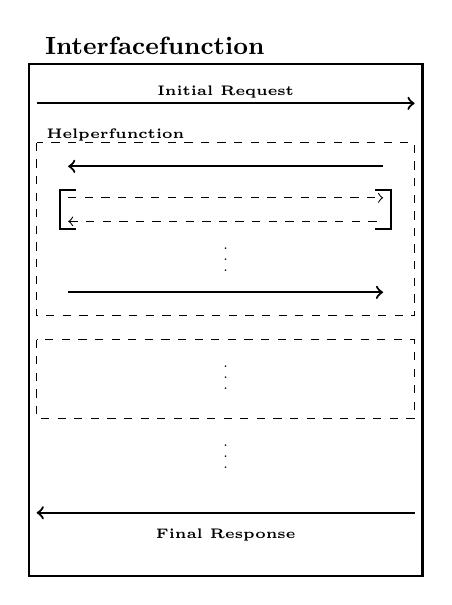
\begin{tikzpicture}[scale=1, every node/.style={scale=1}]
        % Interfacefunktion
        \draw[thick] (0, 6.5) rectangle (5, 0);
        \node[above] at (1.6, 6.5) {\small \textbf{Interfacefunction}};
        \draw[thick,->] (0.1, 6) -- (4.9, 6) node[above,midway,yshift=-2]{\tiny \textbf{Initial Request}};
        \node[below] at (2.5, 2) {\tiny $\vdots$};
        \draw[thick,<-] (0.1, 0.8) -- (4.9, 0.8) node[below,midway,yshift=-2]{\tiny \textbf{Final Response}};

        \draw[dashed] (0.1, 5.5) rectangle (4.9, 3.3);
        \node[above] at (1.1, 5.4) {\tiny \textbf{Helperfunction}};
        \draw[thick,<-] (0.5, 5.2) -- (4.5, 5.2);
        \draw[dashed,->] (0.5, 4.8) -- (4.5, 4.8);
        \draw[dashed,<-] (0.5, 4.5) -- (4.5, 4.5);
        \draw[thick] (0.6, 4.9) -- (0.4, 4.9) -- (0.4, 4.4) -- (0.6, 4.4);
        \draw[thick] (4.4, 4.9) -- (4.6, 4.9) -- (4.6, 4.4) -- (4.4, 4.4);
        \node[below] at (2.5, 4.5) {\tiny $\vdots$};
        \draw[thick,->] (0.5, 3.6) -- (4.5, 3.6);


        \draw[dashed] (0.1, 3) rectangle (4.9, 2);
        \node[below] at (2.5, 3) {\tiny $\vdots$};


        % % Request box
        % \draw[thick] (0, 2.5) rectangle (4, 0);
        % \node[below] at (2, 2.5) {$F_\text{id}$};
        % \draw[thick] (0, 2) -- (4, 2);
        % \node[below] at (2, 2) {$F_\text{argument}(1)$};
        % \draw[dashed] (0, 1.35) -- (4, 1.35);
        % \node[below] at (2, 1.53) {$\vdots$};
        % \draw[dashed] (0, 0.7) -- (4, 0.7);
        % \node[below] at (2, 0.7) {$F_\text{argument}(n)$};
        % \draw[decorate, decoration={brace, amplitude=10pt}] (4.1, 2) -- (4.1, 0)
        %     node[midway, right=10pt] {\text{zmsg\_t}};
        % \draw[decorate, decoration={brace, amplitude=3pt}] (4.1, 2.5) -- (4.1, 2)
        %     node[midway, right=12pt] {\text{Integer}};

    \end{tikzpicture}
    \caption{Die Modularität der Hilfsfunktionen innerhalb einer Interfacefunktion.}
    \label{fig:help_modular}
\end{figure}

Einige Hilfsfunktionen weisen hingegen eine extrem starke Kopplung auf.
Insbesondere ist die Funktion \texttt{mk\_type} hervorzuheben, welche die Typen der in einem Prädikat enthaltenen Elemente konstruiert.
Bei Bedarf dekonstruiert sie den Datentyp von iterierbaren Elementen, wie etwa Listen oder Sets, um an die Typen der wiederum darin enthaltenen Elemente zu gelangen.
Des Weiteren ist die Funktion indirekt rekursiv durch den Aufruf anderer Hilfsfunktionen, welche erneut \texttt{mk\_type} selbst aufrufen.
Die Kopplung zwischen SICStus Prolog und Z3 ist hierbei durch die enthaltenen Bedingungen im Kontrollfluss zusätzlich komplex.
Sowohl die Verwendung von Funktionalitäten der Prolog Bibliothek sowie der Z3-Komponente verändern und bedingen den Verlauf der Methode.
Zur Entkopplung wurde die Logik einer \enquote{State Machine} implementiert, die in verschiedenen Szenarien zusätzliche Informationen
an dem entsprechend anderen Prozess anfordern oder diese an ihn zu senden.
Die Kommunikation macht sich dabei den Statusidentifikator \texttt{UNFINISHED} zu Nutze, um den Prozess über den aktuellen Zustand zu informieren.
Die Funktion wird in den meisten Interfacefunktionen aufgerufen und ist daher ein zentraler Bestandteil des Z3-Interfaces.

In \cref{fig:mk-type-sequence} ist das Sequenzdiagramm der Hilfsfunktion \texttt{mk\_type} dargestellt, welches die Komplexität der Funktion verdeutlicht
und veranschaulicht, wie die Entkopplung der Funktion durchgeführt wurde.
Auf beiden Seiten des Diagramms sind die ProB- und Z3-Prozesse abgebildet, die schrittweise ihren Zustand ändern, welchen sie durch die Nachrichtenübermittlung synchron halten.
Zunächst wird überprüft, ob der Typ ein Atom ist, wie \texttt{integer}, \texttt{real} oder \texttt{boolean}.
Wenn dies nicht der Fall ist, wird überprüft, ob der Typ bereits zuvor konstruiert wurde.
Sollte er nicht existieren, wird der Typ dekonstruiert. Die Dekonstruktion unterscheidet zwischen den Typen \texttt{set}, \texttt{global}, \texttt{couple} und \texttt{record}.
\todo{state machine farblich oder so}
\begin{figure}[!htp]
  \centering
  \begin{tikzpicture}[scale=3, every node/.style={scale=0.7}]
    % \node at (1,5.4) {\textbf{Sequenz Diagramm der Hilfsfunktion $mk\_type$}};

    \begin{scope}
      \clip (-1,1.3) rectangle (3,5.5);

      \coordinate (a) at (0,0);
      \coordinate (b) at (0,5);
      \coordinate (c) at (2,0);
      \coordinate (d) at (2,5);


      \draw (a) -- (b) node[pos=1.03]{\large \textbf{ProB-Client}};
      \draw (c) -- (d) node[pos=1.03]{\large \textbf{Z3-Server}};

      \node[left] at ($(a)!0.955!(b)$) {check if type is atom};
      \node[right] at ($(c)!0.925!(d)$) {check if type exists};
      \node[left] at ($(a)!0.89!(b)$) {return};
      \node[right] at ($(c)!0.87!(d)$) {return};
      \node[left] at ($(a)!0.805!(b)$) {check prolog term};
      \node[right] at ($(c)!0.775!(d)$) {check if type exists};
      \node[left] at ($(a)!0.74!(b)$) {return};
      \node[right] at ($(c)!0.72!(d)$) {return};
      \node[left] at ($(a)!0.685!(b)$) {check iterable type};
      \node[left] at ($(a)!0.56!(b)$) {return};
      \node[right] at ($(c)!0.54!(d)$) {return};

      \draw[stealth-] ($(a)!0.96!(b)$) -- node[above,sloped,midway]{} ($(c)!0.98!(d)$);
      \draw[-stealth] ($(a)!0.95!(b)$) -- node[above,sloped,midway]{it is} ($(c)!0.93!(d)$);
      \draw[stealth-] ($(a)!0.90!(b)$) -- node[above,sloped,midway]{it does} ($(c)!0.92!(d)$);
      \draw[-stealth] ($(a)!0.89!(b)$) -- node[above,sloped,pos=0.4]{} ($(c)!0.87!(d)$);

      \draw[-stealth] ($(a)!0.95!(b)$) -- node[below,sloped,pos=0.1]{it is not} ($(c)!0.84!(d)$);
      \draw[stealth-] ($(a)!0.81!(b)$) -- node[above,sloped,midway]{} ($(c)!0.83!(d)$);
      \draw[stealth-] ($(a)!0.81!(b)$) -- node[above,sloped,pos=0.2]{it does not} ($(c)!0.92!(d)$);

      \draw[-stealth] ($(a)!0.80!(b)$) -- node[above,sloped,midway]{} ($(c)!0.78!(d)$);
      \draw[stealth-] ($(a)!0.75!(b)$) -- node[above,sloped,midway]{it does} ($(c)!0.77!(d)$);
      \draw[-stealth] ($(a)!0.74!(b)$) -- node[above,sloped,midway]{} ($(c)!0.72!(d)$);

      \draw[stealth-] ($(a)!0.69!(b)$) -- node[above,sloped,pos=0.2]{it does not} ($(c)!0.77!(d)$);
      \draw[-stealth] ($(a)!0.68!(b)$) -- node[above,sloped,midway]{} ($(c)!0.66!(d)$);
      \draw[stealth-] ($(a)!0.63!(b)$) -- node[above,sloped]{} ($(c)!0.65!(d)$);

      \path[draw,dashed,->] ($(a)!0.68!(b)$) arc[start angle=270, end angle=90, radius=0.75] node[pos=0.4, right]{set};
      \path[draw,dashed,->] ($(c)!0.65!(d)$) arc[start angle=270, end angle=450, radius=0.85] node[pos=0.3, left]{set};

      \draw[-stealth] ($(a)!0.62!(b)$) -- node[above,sloped,midway]{global atom} ($(c)!0.60!(d)$);
      \draw[stealth-] ($(a)!0.57!(b)$) -- node[above,sloped,midway]{} ($(c)!0.59!(d)$);
      \draw[-stealth] ($(a)!0.56!(b)$) -- node[above,sloped,midway]{} ($(c)!0.54!(d)$);

      \draw[-stealth] ($(a)!0.62!(b)$) -- node[above,sloped,pos=0.65]{couple} ($(c)!0.52!(d)$);
      \draw[stealth-] ($(a)!0.49!(b)$) -- node[above,sloped]{} ($(c)!0.51!(d)$);
      \draw[-stealth] ($(a)!0.48!(b)$) -- node[above,sloped]{} ($(c)!0.46!(d)$);

      \path[draw,dashed,->] ($(a)!0.48!(b)$) arc[start angle=270, end angle=90, y radius=1.25, x radius=1] node[pos=0.33, right]{couple elements};
      \path[draw,dashed,->] ($(c)!0.46!(d)$) arc[start angle=270, end angle=450, y radius=1.325, x radius=1] node[pos=0.35, left]{couple elements};

      \draw[-stealth] ($(a)!0.62!(b)$) -- node[above,sloped,pos=0.55]{record} ($(c)!0.44!(d)$);
      \draw[stealth-] ($(a)!0.41!(b)$) -- node[above,sloped]{} ($(c)!0.43!(d)$);
      \draw[-stealth] ($(a)!0.40!(b)$) -- node[above,sloped]{next list element} ($(c)!0.38!(d)$);
      \draw[stealth-] ($(a)!0.35!(b)$) -- node[above,sloped]{} ($(c)!0.37!(d)$);
      \draw[-stealth] ($(a)!0.34!(b)$) -- node[above,sloped]{} ($(c)!0.32!(d)$);
      \draw[stealth-] ($(a)!0.29!(b)$) -- node[above,sloped]{} ($(c)!0.31!(d)$);
      \draw[-stealth] ($(a)!0.40!(b)$) -- node[above,sloped,pos=0.55]{list empty} ($(c)!0.27!(d)$);

      \path[draw,dashed,->] ($(a)!0.29!(b)$) arc[start angle=270, end angle=90, y radius=0.285, x radius=0.3] node[midway, left]{};
      \path[draw,dashed,->] ($(c)!0.31!(d)$) arc[start angle=270, end angle=450, y radius=0.16, x radius=0.3] node[midway, right]{};

      \path[draw,dashed,->] ($(a)!0.40!(b)$) arc[start angle=270, end angle=90, y radius=1.45, x radius=1] node[midway, left]{};
      \path[draw,dashed,->] ($(c)!0.27!(d)$) arc[start angle=270, end angle=450, y radius=1.8, x radius=1] node[midway, right]{};

    \end{scope}

  \end{tikzpicture}
  \caption{Das Sequenzdiagramm der Hilfsfunktion \texttt{mk\_type}. Der Übersicht halber sind nicht alle Nachrichten beschriftet. Derartige Nachrichten übermitteln zumeist ausschließlich Statusindikatoren.}
  \label{fig:mk-type-sequence}
\end{figure}

\subsubsection{Optimierungen}
\label{subsec:optimizations}

Nach der erfolgreichen Portierung der Schnittstelle und der Implementierung aller notwendigen Funktionen
lassen sich zusätzlich kleine Optimierungen und Verbesserungen vornehmen, um Effizienz, Lesbarkeit und Wartbarkeit des Codes zu erhöhen.
\todo{string vektor dafuq}
Eine der elementarsten Optimierungsmöglichkeiten ist die Vermeidung von Nachrichtenaustausch beider Prozesse
innerhalb von Schleifen. Dieses Verhalten tritt insbesondere dann auf, wenn Prolog Datenstrukturen übermittelt werden,
die iterierbar sind, wie Listen, Vektoren und Records.
In diesen Fällen wird für jedes Element der Struktur eine Nachricht an den Server gesendet,
um das aktuelle Element zu übermitteln.
Dieses Verhalten kann in einzelnen Fällen durch die Übermittlung der gesamten Struktur in einer einzigen Nachricht vermieden werden.
Beispielsweise lässt sich eine Prolog Liste zunächst in einem String Vektor akkumulieren,
um anschließend in einer einelnen Nachricht an den Server gesendet zu werden.
\todo{verständlichere erklärung}
Eine weitere Optimierungsmöglichkeit ist die Vermeidung von unnötigen Nachrichten an den Server.
Beispielsweise illustriert \cref{lst:unnecessary-ctx-data} vermeidbare Komplexität durch die Verwendung unnötiger Datenobjekte.
Anhand der Variablen \texttt{translation\_type\_atom} wird das Objekt \texttt{ctx\_data} ermittelt, welches an die Funktion \texttt{prolog\_type\_list\_to\_sort\_vector} übergeben wird.
Diese verwendet das Objekt ausschließlich zur Ermittlung der Variablen \texttt{translation\_type\_atom}. Das Problem hierbei ist,
dass \texttt{ctx\_data} in der neuen Architektur auf der Seite des Server-Prozesses liegt und somit einen Nachrichtenaustausch erfordert.
Die Problematik lässt sich umgehen, indem die Funktion \texttt{prolog\_type\_list\_to\_sort\_vector} dahingehen refaktorisiert wird,
direkt mit \texttt{translation\_type\_atom} aufgerufen zu werden oder sogar gänzlich darauf zu verzichten.

\begin{lstlisting}[
    float, caption={Illustrationsbeispiel zur Optimierung von vermeidbarer Objektkomplexität.}, label={lst:unnecessary-ctx-data}, language=C++
  ]
  // function: mk_op_comprehension_set_multi
  ContextData ctx_dta =
    get_translation_representant_ctx_data(translation_type_atom);
  prolog_type_list_to_sort_vector(ctx_data, couple_types);
  // ...

  // function: prolog_type_list_to_sort_vector
  mk_sort(ctx_data->get_translation_type_atom());
\end{lstlisting}

Zuletzt wurde das DRY\footnote{Don't Repeat Yourself}-Prinzip angewendet, um die Wartbarkeit des Codes zu erhöhen,
indem gewisse Hilfsfunktionen ausschließlich auf entweder der Prolog- oder der Serverseite implementiert wurden.
Der ursprüngliche Kontrollfluss verlangte zum Beispiel die Implementierung einzelner Hilfsfunktionen
in beiden Prozessen. Durch die Anwendung des Programmierprinzips und minimaler Anpassung im Quellcode wurden diese Funktionen ausschließlich innerhalb eines Prozesses implementiert.

\subsubsection{Serveranbindung}
\label{subsec:server-connection}

Der Z3-Prozess wird nicht manuell gestartet, sondern,
um eine angenehme Nutzerfreundlichkeit zu gewährleisten, automatisch im Z3-Interface als Subprozess von ProB erzeugt.
Insbesondere bedeutet das, dass der Z3-Server ausschließlich auf Anfrage von ProB gestartet wird, wenn das entsprechende Interface verwendet wird.
Als Subprozess wird der Z3-Solver mit der Beendigung von ProB ebenfalls terminiert.
Dieses Verhalten ist innerhalb der Prolog-Seite des Z3-Interfaces implementiert und wird durch das Prädikat \texttt{init\_z3interface} realisiert, welches dahingehend erweitert wurde.
Die Implementierung des Prädikats ist in \cref{lst:init-z3interface} gezeigt.

\begin{lstlisting}[
  float, caption={Das Prädikat zur Initialisierung des Z3-Interfaces.}, label={lst:init-z3interface}, language=Prolog
]
init_z3interface :- is_initialised(_), !.
init_z3interface :-
    catch(load_foreign_resource(library(z3interface)),E,
          (format(user_error,'*** LOADING Z3 library failed~n',[]),
           assert(z3_init_exception(E)),
           fail)
          ),
    get_path_to_fresh_z3_endpoint(Endpoint),
    process_create('./lib/z3rver', [Endpoint], [stdout(null)]),
    init(Endpoint, Zocket),
    assertz(is_initialised(Zocket)).
\end{lstlisting}

Der Endpoint zur ZeroMQ Kommunikation wird generiert
und als Funktionsargument an die \texttt{init} Funktion übergeben, welche die Verbindung zum Z3-Server herstellt (Z. 8\texttt{-}10).
Die Funktion \texttt{process\_create} wird eingesetzt, um den Z3-Server als Subprozess zu starten,
welcher durch die Verwendung der Systemargumente ebenfalls über den generierten Endpoint informiert wird.
So sind beide Prozesse in Kenntnis desselben Endpoints und können miteinander kommunizieren.
Der Endpoint selbst ist hierbei effektiv ein Pfad zu einer temporären Datei, die als Kommunikationskanal zwischen den Prozessen dient.
Er wird als einzigartiger Dateiname innerhalb von \texttt{get\_path\_to\_fresh\_z3\_endpoint} generiert.

\subsubsection{Logging}
\label{subsec:logging}

Der Z3-Server wurde mit einem Logging-System ausgestattet, um die potentielle Fehlersuche und -behebung zu erleichtern.
Insbesondere hilft das Logging-System dabei, eine klare Übersicht über den Verlauf des Servers zu erhalten und damit die Nachvollziehbarkeit zu erhöhen.
Durch das Protokollieren von Ereignissen, wie etwa dem Empfangen und Senden von Nachrichten, der aktuellen Funktion, die ausgeführt wird, sowie dem Auftreten von Fehlern,
wird gewährleistet, dass das Serververhalten transparent und ersichtlich ist.
Derartige Informationen erleichtern auch die zukünftige Wartung und Erweiterung des Systems.
Innerhalb des Prolog Prädikates \texttt{process\_create} lässt sich die Ausgabe des Z3-Servers allerdings nur schwer kontrollieren und verlangt die Verwendung der standard shell (sh).
Aus diesem Grund wurde das Logging-System auf der Seite des Z3-Servers selbst implementiert, um gegebenenfalls die Ausgabe in einer Datei zu speichern.
Die Implementierung funktioniert durch das Umleiten des Standardausgabestreams in einen eigenen Dateideskriptor.
Dieser Dateideskriptor zeigt bei Verwendung des Logging-Systems in eine valide Datei im aktuellen Dateiverzeichnis.
Sollte das Logging-System nicht verwendet werden, wird der Standardausgabestream auf \enquote{/dev/null} umgeleitet, um die Ausgabe zu unterdrücken.
Somit lässt sich über die Systemargumente beim Start des Servers entscheiden, ob das Logging-System aktiviert werden soll oder nicht.
Zur Aktivierung muss lediglich \cref{lst:init-z3interface} so angepasst werden, dass neben dem Endpoint (Z. 9) zusätzlich das Argument \enquote{\texttt{-}\texttt{-}log} an den Server übergeben wird.

Da die Erweiterbarkeit des Systems gewährleistet werden soll, muss beachtet werden, dass der Z3-Server in eine Datei schreibt, die einzigartig zu seinem Prozess ist.
Sollten in Zukunft mehrere Z3-Prozesse existieren, würden diese andernfalls in dieselbe Datei schreiben und die Logausgabe dadurch unübersichtlich machen.
Womöglich könnte dies auch zu Konflikten führen, wenn mehrere Prozesse gleichzeitig in dieselbe Datei schreiben, sodass Informationen vollständig verloren gehen oder nur ein einziger Z3-Solver die Datei beschreiben kann.
Um dies zu verhindern, wird der Dateiname der Logdatei durch den Endpoint des Z3-Servers ergänzt.
Beispielsweise schreibt der Z3-Solver bei einem Endpoint \texttt{ipc:///tmp/z3rver96485092.probz} in die Datei \texttt{z3rver96485092.probz.log}.

\subsubsection{Exceptions}
\label{subsec:exceptions}

Die korrekte Behandlung von Exceptions ist ein wichtiger Bestandteil der Implementierung, um die Stabilität des Systems zu gewährleisten.
Sie ist jedoch grundlegend fehleranfällig und kann zu unerwarteten Abstürzen führen, wenn sie nicht ordnungsgemäß behandelt wird.
Die Struktur der neuen Architektur fügt dem Behandlungsprozess von Exceptions eine zusätzliche Komplexität hinzu, da die ProB- und Z3-Prozesse unabhängig voneinander auf Fehler stoßen können.
Beim Auftreten einer Exception in einem der Prozesse muss der andere Prozess über den Fehler informiert werden, um eine entsprechende Fehlerbehandlung durchzuführen.
Hierbei ist zu beachten, dass das Kommunikationsmuster der beiden Prozesse eingehalten werden muss, wenn eine Exception auftritt.
Dies ist nicht trivial, da Exceptions den natürlichen Kontrollfluss fundamental verändern.

% Wenn eine Exception geworfen wird, verlässt der Kontrollfluss einer Anwendung grundsätzlich den aktuellen Codeblock und propagiert aufwärts im Funktionsaufruf-Stack (engl. \enquote{Call Stack}),
% bis ein passender Exception-Handler gefunden wird, der den Fehler behandelt oder das Programm terminiert.
Zusätzliche Schwierigkeiten entstehen durch das Z3-Interface von SICStus Prolog auf der Seite des ProB-Prozesses,
da die Schnittstelle einen durch \texttt{SP\_raise\_exception} geworfenen Fehler als ausstehend (engl. \enquote{pending}) behandelt und den Kontrollfluss nicht wie gewöhnlich unterbricht.
Stattdessen wird der Fehler also zwischengespeichert und erst bei der Rückkehr aus der Interfacefunktion nach Prolog behandelt.

In der originalen Architektur des Z3-Interfaces existiert keine klare Struktur zur Behandlung von Exceptions.
Beispielsweise haben manche Hilfsfunktionen ihre eigenen Exception-Handler, die im Falle eines Fehlers einen nicht-validen Wert (wie etwa \texttt{nullptr}) zurückgeben.
Dieser Wert wird in gewissen Interfacefunktionen nicht überprüft, was zu unerwarteten Abstürzen führen kann, wenn die entsprechende Exception auftritt.
Manche Funktionen implementieren einen Exception-Handler für den gesamten Funktionskörper, andere hingegen nur für einzelne Codeblöcke, die teilweise nicht alle Fehlerfälle abdecken.
Ebenfalls existieren Interfacefunktionen (wie etwa \texttt{mk\_sort} oder \texttt{mk\_record\_field}), die keine Fehlerbehandlung implementieren und somit bei einem Fehler unerwartet (mit einem Segmentation Fault) terminieren.

Aus diesen Gründen wurde das Exception-Handling in der neuen Architektur des Z3-Interfaces grundlegend überarbeitet.
Die Exception-Handler wurden konsistent in allen Interfacefunktionen implementiert, sodass der gesamte Funktionskörper abgedeckt ist.
Auch wenn große Codeblöcke innerhalb eines Try-Catch-Blocks einen unschönen Codestyle darstellen,
ist so gewährleistet, dass nicht nur alle Fehler, sondern auch daraus resultierende Folgefehler abgefangen werden.
Entsprechend wurden die Hilfsfunktionen so refaktorisiert, dass sie selbst keine Exceptions mehr abfangen, sondern diese an die aufrufende Funktion weiterreichen.
Die aufrufende Funktion ist nach einer endlichen Propagierung zwangsläufig eine Interfacefunktion, welche den Fehler somit abfängt und entsprechend behandelt.

\begin{lstlisting}[
  float, caption={Der Exception-Handler des Z3-Prozesses.}, label={lst:z3-exception-handler}, language=C++
]
void raise_Z3_exception(const z3::exception& e, std::string name) {
  fprintf(logFile, "[ERROR] z3_exception in %s : %s\n",
   name.c_str(), e.msg());
  if (z3exc_occured) {
      return;
  }
  z3exc_occured = true;
  zmsg_t *response = zmsg_new();
  zmsg_addstr(response, e.msg());
  zmsg_addstr(response, name.c_str());
  send_z3_response(Z3Status::NOK, &response);
}
\end{lstlisting}

Um die Einhaltung des Request-Reply-Modells zu garantieren, wurde ein spezieller Exception-Handler in dem Z3-Prozess implementiert.
Dieser wird immer aufgerufen, wenn eine Exception in einer der Interfacefunktionen auftritt und leitet den Fehler gegebenenfalls an den ProB-Prozess weiter.
Die Implementierung des Exception-Handlers ist in \cref{lst:z3-exception-handler} gezeigt.
Insbesondere ist auf die Variable \texttt{z3exc\_occured} zu achten, die verhindert, dass mehrere Exceptions an den ProB-Prozess gesendet werden, bevor der erste Fehler behandelt wurde.
Entsprechend wird auch in \cref{lst:server-structure} die schlussendliche Antwort einer Anfrage nur dann gesendet, wenn keine Exception aufgetreten ist (Z. 25).
Es ist nämlich davon auszugehen, dass der Fehler innerhalb des ProB-Prozesses in diesem Fall bereits behandelt wurde und die Interfacefunktion dort verlassen worden ist.
Somit würde eine weitere Nachricht gegen das Kommunikationsmuster verstoßen und zu unerwarteten Fehlern führen.

Als grundlegende Konvention sollte der Z3-Server nach dem Senden einer Antwort und vor dem Erhalten der nächsten Anfrage keinen Code ausführen, der Fehler verursachen könnte.
Andernfalls könnte der ProB-Prozess nicht über die Exception in Kenntnis gesetzt werden, da der Z3-Server in diesem Fall nicht mehr in der Lage wäre, eine Nachricht zu senden.

\subsection{Kompilierung}

Nach der vollständigen Umsetzung der neuen Systemarchitektur muss sowohl das Z3-Interface als auch der Z3-Solver kompiliert werden.
Hierzu wurden Änderungen im Makefile der Programmerweiterung von ProB vorgenommen.

\subsubsection{Makefile}

Das eigentliche Z3-Interface wird als Bibliothek in Form einer dynamischen Shared Library kompiliert.
Dieses Verhalten ändert sich nicht, es müssen lediglich minimale Anpassungen vorgenommen werden, wie das Entfernen der Z3- und das Hinzufügen der ZMQ-Bibliothek.
Durch das Importieren der \texttt{shared\_libs.mk} Datei in das Makefile wird die Kompilierung der Interface-Bibliothek mithilfe der \texttt{install} Regel automatisiert.

Es wird eine weitere Regel definiert, welche die Kompilierung des Z3-Solvers durchführt und die resultierende Binärdatei in das Zielverzeichnis kopiert.
Diese Regel wird als Abhängigkeit von \texttt{install} hinzugefügt.
Die Implementierung der Regel ist in \cref{lst:makefile} gezeigt.
Es ist zu beachten, dass die Abhängigkeiten \texttt{\$(LIBCZMQ\_PATH)} und \texttt{\$(target\_dir)/\$(LIBZ3)} sicherstellen,
dass sowohl die ZeroMQ- als auch die Z3-Bibliothek vor der Kompilierung des Z3-Solvers vorhanden sind und entsprechend korrekt eingebunden werden können.
Der resultierende Befehl, welcher durch das Makefile ausgeführt wird, ist in \cref{lst:command} gezeigt.

\begin{lstlisting}[
  float, caption={Ausschnitt des Makefiles zur Kompilierung des Z3-Solvers.}, label={lst:makefile}, language=sh
]
include ../shared_libs.mk

$(target_dir)/z3rver: z3rver
  cp -f z3rver $@

z3rver: $(LIBCZMQ_PATH) $(target_dir)/$(LIBZ3)
        $(z3solver_files) $(z3solver_header)
  $(CXX) $(Z3CXXFLAGS) $(Z3LDFLAGS) $(z3solver_files)
   $(Z3LDLIBS) -o z3rver

install: $(target_dir)/z3rver
\end{lstlisting}

\begin{lstlisting}[
  float, caption={Der Kompilierungsbefehl.}, label={lst:command}, language=sh
]
g++ -std=gnu++11  -Wall -O2 -g -I../zmq_lib/prefix/include
 -I./shared -I./prefix/include -DZ3VERS="4.13.2"
 -L../zmq_lib/prefix/lib -L./prefix/bin -Wl,-rpath,'$ORIGIN'
 z3server/context_data.cpp z3server/z3rver.cpp -lczmq -pthread -lz3
 -o z3rver
cp -f z3rver ../../lib/z3rver
\end{lstlisting}

Nach Abschluss der Implementierung und Kompilierung konnten alle vorhandenen Tests zur Überprüfung der Funktionalität des Z3-Interfaces erfolgreich durchgeführt werden.
Dies bestätigt, dass die Architekturänderung erfolgreich umgesetzt wurde.
